\documentclass{beamer}

%% \documentclass[handout]{beamer}
%% % use this with the [handout] option to create handouts for the audience
%% \usepackage{pgfpages}
%% \pgfpagesuselayout{2 on 1}[a4paper,border shrink=5mm]

\mode<presentation>
{
  \usetheme{Diku}
% set this to your preferences:
  \setbeamercovered{invisible}
%  \setbeamercovered{transparent}
}

\usepackage{graphicx}
\usepackage{epic}

\usepackage{amsmath}
\usepackage{amssymb}
\usepackage{amsthm}

\newcommand{\basetop}[1]{\vtop{\vskip-1ex\hbox{#1}}}
\newcommand{\source}[1]{\let\thefootnote\relax\footnotetext{\scriptsize\textcolor{kugray1}{Source: #1}}}

% for coloured code citation in text:
\usepackage{fancyvrb}

%%%%%%%%%%%%%%%%%%%%%%%%%%%%%%%%%
%%%%%    code sections   %%%%%%%%
%%%%%%%%%%%%%%%%%%%%%%%%%%%%%%%%%

% code highlighting commands in own block
\DefineVerbatimEnvironment{code}{Verbatim}{fontsize=\scriptsize}
\DefineVerbatimEnvironment{icode}{Verbatim}{fontsize=\scriptsize}

% Fancy code with color commands:
\DefineVerbatimEnvironment{colorcode}%
        {Verbatim}{fontsize=\scriptsize,commandchars=\\\{\}}

%%%%%%%%%%%%%%%%%%%%%%%%%%%%%%%%%%
%%%%%    some coloring    %%%%%%%%

\definecolor{Red}{RGB}{220,50,10}
\definecolor{Blue}{RGB}{0,51,102}
\definecolor{Yellow}{RGB}{102,51,0}
\definecolor{Orange}{RGB}{178,36,36}
\definecolor{Grey}{RGB}{180,180,180}
\definecolor{Green}{RGB}{20,120,20}
\definecolor{Purple}{RGB}{160,50,100}
\newcommand{\red}[1]{\textcolor{Red}{{#1}}}
\newcommand{\blue}[1]{\textcolor{Blue}{{#1}}}
\newcommand{\yellow}[1]{\textcolor{Yellow}{{#1}}}
\newcommand{\orange}[1]{\textcolor{Orange}{{#1}}}
\newcommand{\grey}[1]{\textcolor{Grey}{{#1}}}
\newcommand{\green}[1]{\textcolor{Green}{{#1}}}
\newcommand{\purple}[1]{\textcolor{Purple}{{#1}}}




% use "DIKU green" from our color theme for \emph
\renewcommand{\emph}[1]{\textcolor{structure}{#1}}
% use some not-too-bright red for an \emp command
\definecolor{DikuRed}{RGB}{130,50,32}
\newcommand{\emp}[1]{\textcolor{DikuRed}{ #1}}
\definecolor{CosGreen}{RGB}{10,100,70}
\newcommand{\emphh}[1]{\textcolor{CosGreen}{ #1}}
\definecolor{CosBlue}{RGB}{55,111,122}
\newcommand{\emphb}[1]{\textcolor{CosBlue}{ #1}}
\definecolor{CosRed}{RGB}{253,1,1}
\newcommand{\empr}[1]{\textcolor{CosRed}{ #1}}

\newcommand{\mymath}[1]{$ #1 $}
\newcommand{\myindx}[1]{_{#1}}
\newcommand{\myindu}[1]{^{#1}}

\newcommand{\Fasto}{\textsc{Fasto}\xspace}


%%%%%%%%%%%%%%%%%%%%

\title[Interconnect]{Scalable Cache Coherence \& Interconnect}

\author[C.~Oancea]{Cosmin E. Oancea {\tt cosmin.oancea@diku.dk}}

\institute{Department of Computer Science (DIKU)\\University of Copenhagen}


\date[Sept 2014]{September 2014 PMPH Lecture Notes}


\begin{document}

\titleslide

\begin{frame}
\frametitle{Structure of a Compiler}

\begin{tabular}{ccc}
Program text&&\\
$\downarrow$ &&\\
\framebox{Lexical analysis} && Binary machine code\\
$\downarrow$ && $\uparrow$ \\
Symbol sequence && \textcolor{gray}{\framebox{Assembly and linking}} \\
$\downarrow$ && $\uparrow$ \\
\framebox{Syntax analysis} && Ditto with named registers\\
$\downarrow$ && $\uparrow$ \\
Syntax tree && \framebox{Register allocation} \\
$\downarrow$ && $\uparrow$ \\
\red{\framebox{Type Checking}} && Symbolic machine code\\
$\downarrow$ &&  $\uparrow$ \\
Syntax tree  && \framebox{Machine code generation} \\
$\downarrow$ && $\uparrow$ \\
\framebox{Intermediate code generation} &$\longrightarrow$ & Intermediate code
\end{tabular}

\end{frame}



%%%%%%%%%%%%%%%%%%%%%%%%%%%%%%%%%%%%%%%%%%%%%%%%%%%%%%%%%%%%%%%%%%%%%%
%%%%%%%%%%%%%%%%%%%%%%%%%%%%%%%%%%%%%%%%%%%%%%%%%%%%%%%%%%%%%%%%%%%%%%
%%%%%%%%%%%%%%%%%%%%%%%%%%%%%%%%%%%%%%%%%%%%%%%%%%%%%%%%%%%%%%%%%%%%%%
\begin{frame}[fragile]
	\tableofcontents
\end{frame}

%%%%%%%%%%%%%%%%%%%%%%%%%%%%%%%%%%%%%%%%%%%%%%%%%%%
%%%%%%%%%%%%%%%%%%%%%%%%%%%%%%%%%%%%%%%%%%%%%%%%%%%
%%%%%%%%%%%%%%%%%%%%%%%%%%%%%%%%%%%%%%%%%%%%%%%%%%%

\section{Scalable Shared Memory Systems}

\begin{frame}[fragile,t]
\frametitle{Bus-Based SMPs Do Not Scale}

\emph{Ideally, memory bandwidth should scale linearly with the number of nodes,
and memory latency should remain constant}.\bigskip

\alert{Bus-Based Multiprocessors are inherently NON-Scalable}:\medskip
\begin{itemize}
    \item \emp{Bus Bandwidth} capped by {\tt (\# of bus wires)$\times$clockrate}, and
    \item \emp{actually decreases as more noded are added}, 
            because the wire length and the load on them 
            increases with the number of nodes.\bigskip
    \item Dance Hall: memory latency about the same for any access,
            but as the \# of procs goes up, the latency of all
            accesses increases.\bigskip
    \item \emp{Snoopy (Broadcast) Based Protocols are NOT Scalable},
            because involve {\em all} nodes in {\em all} coherence transactions. 
\end  {itemize}
\end{frame}

\begin{frame}[fragile,t]
\frametitle{cc-NUMA: Cache Coherent Non-Uniform Mem Arch}

\emph{Def. Scalable: memory bandwidth should grows linearly and
memory access latency grows sub-linearly with the number of nodes}.
%\vspace{-5ex}
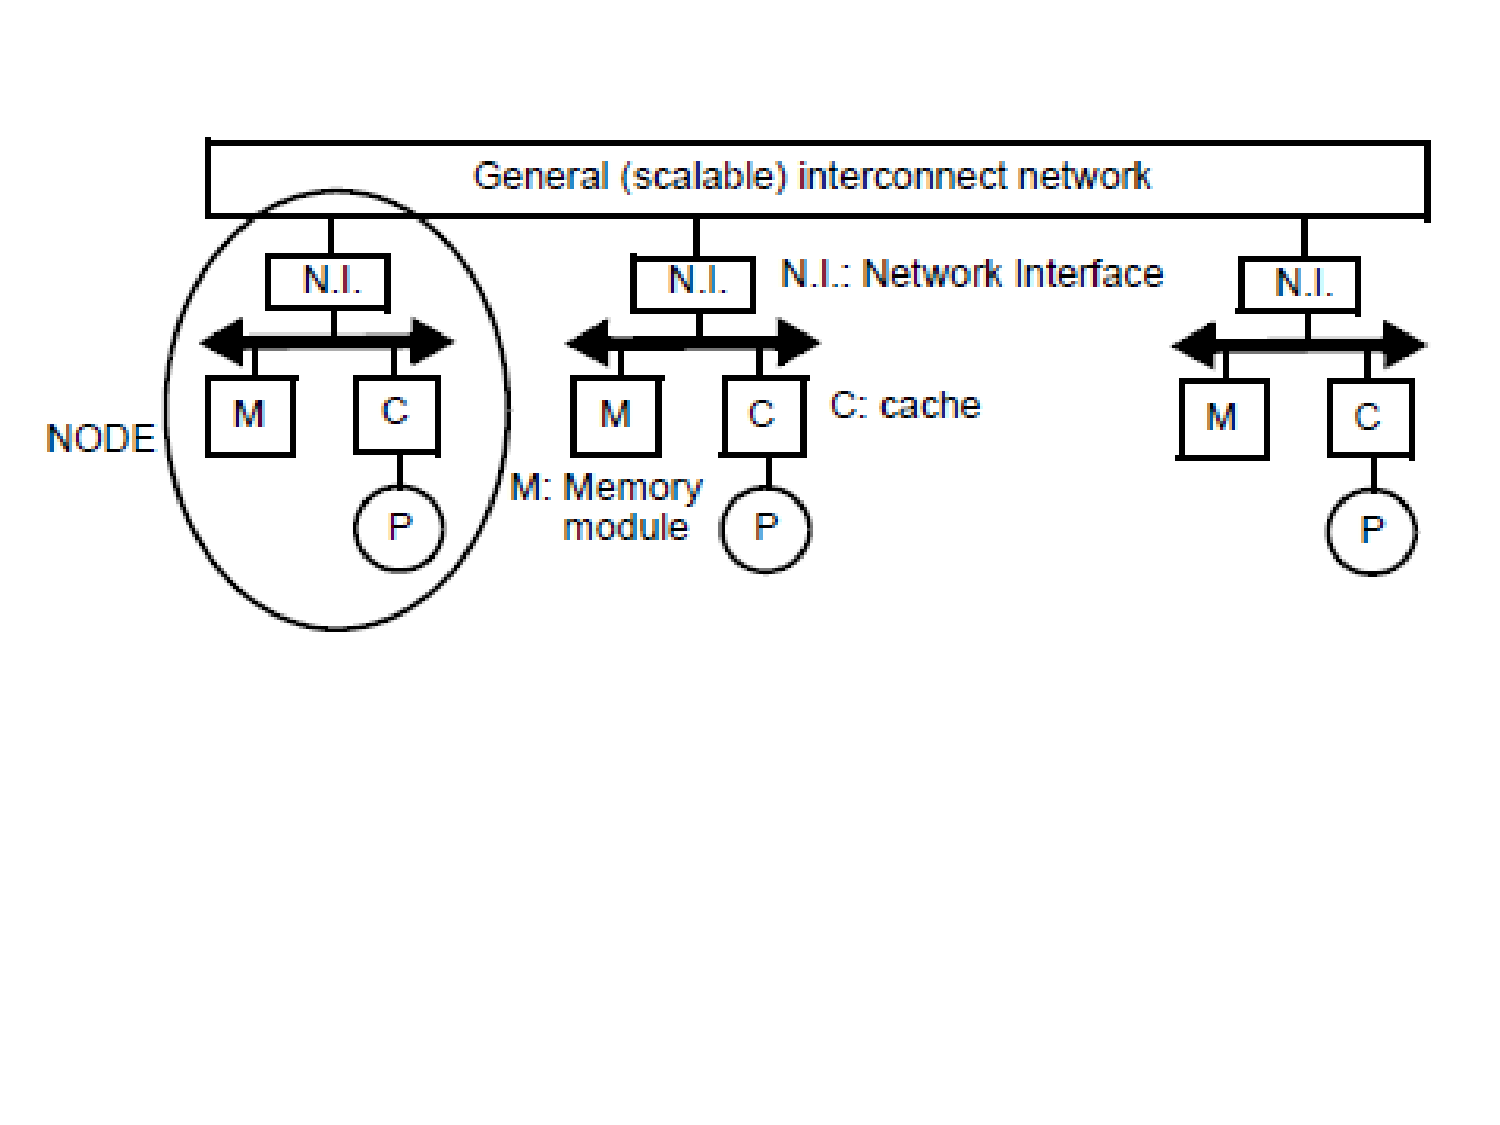
\includegraphics[width=59ex]{FigsInfCoherence/MultiNode}
\vspace{-20ex}

\emph{cc-NUMA} because latency of a local mem module is $<$ of a remote:\\
\begin{itemize}
    \item Memory partitioned into banks \& distributed across nodes 
            to leverage locality. Can be Main Mem or shared cache (NUCA).
    \item Uses a scalable interconnect to accomodate bandwidth,
    \item \emph{Uses scalable directory protocols to keep track of sharing.}
\end  {itemize}

\end{frame}

\begin{frame}[fragile,t]
\frametitle{Hardware Structure for Baseline Directory Protocol}

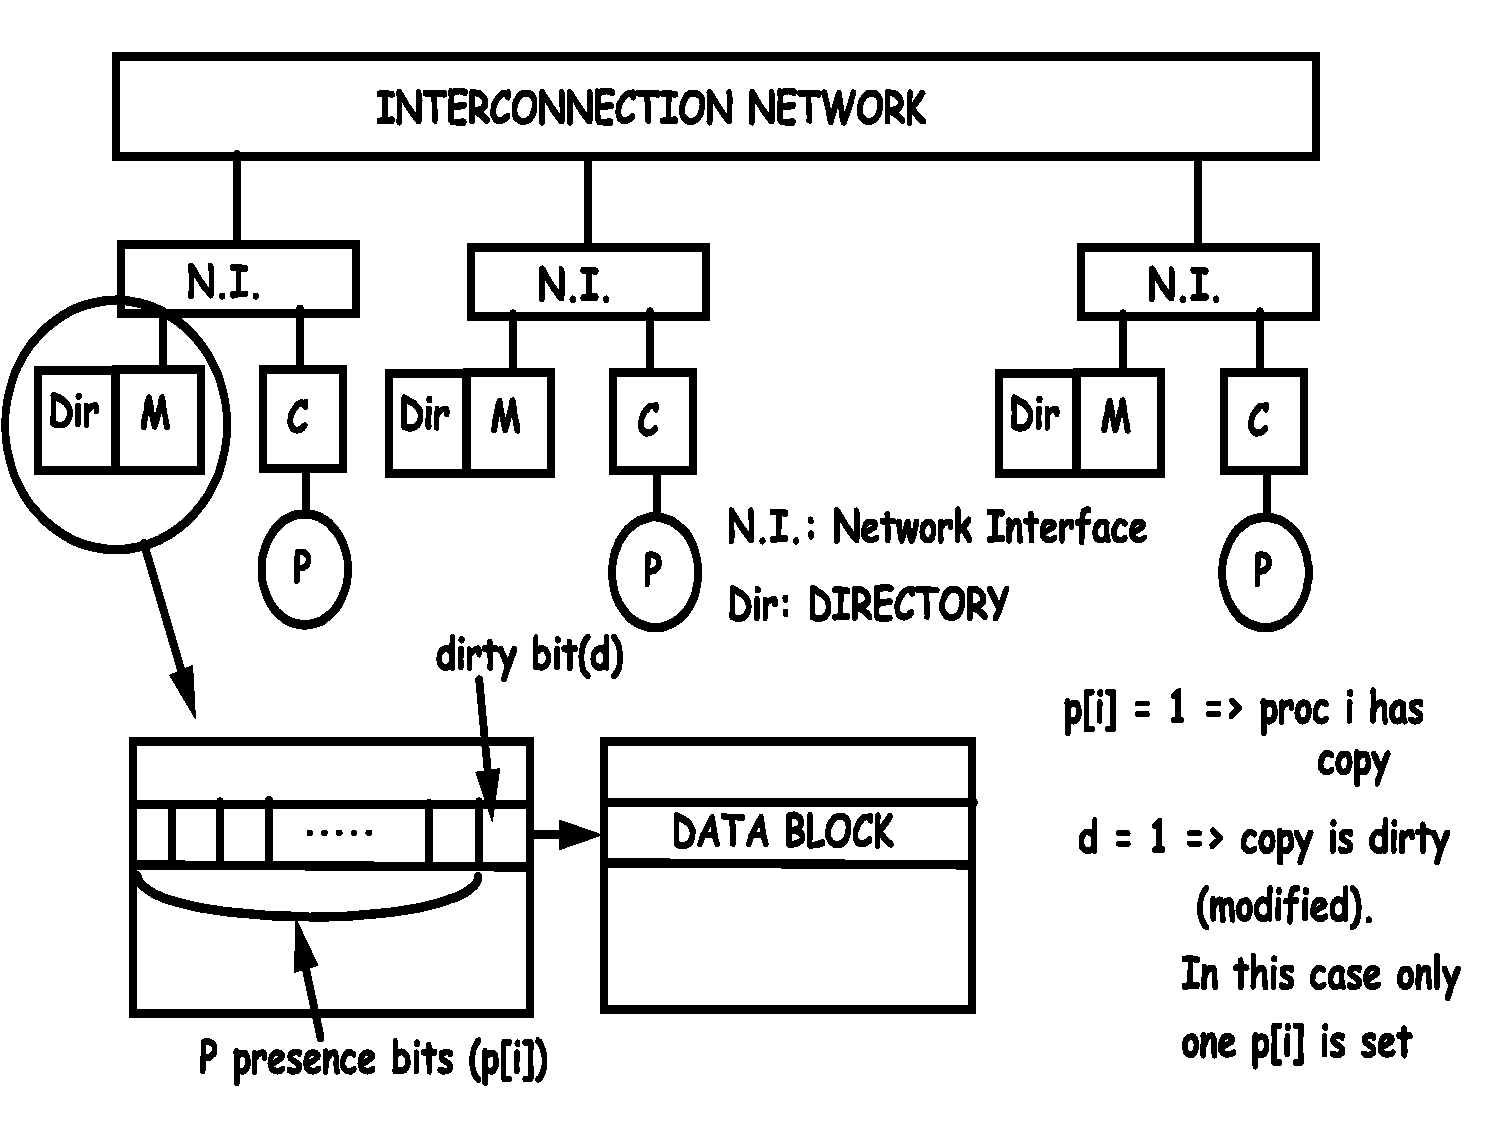
\includegraphics[width=59ex]{FigsInfCoherence/DirBasedProt}

\end{frame}

\begin{frame}[fragile,t]
\frametitle{Presence-Flag Vector Scheme}

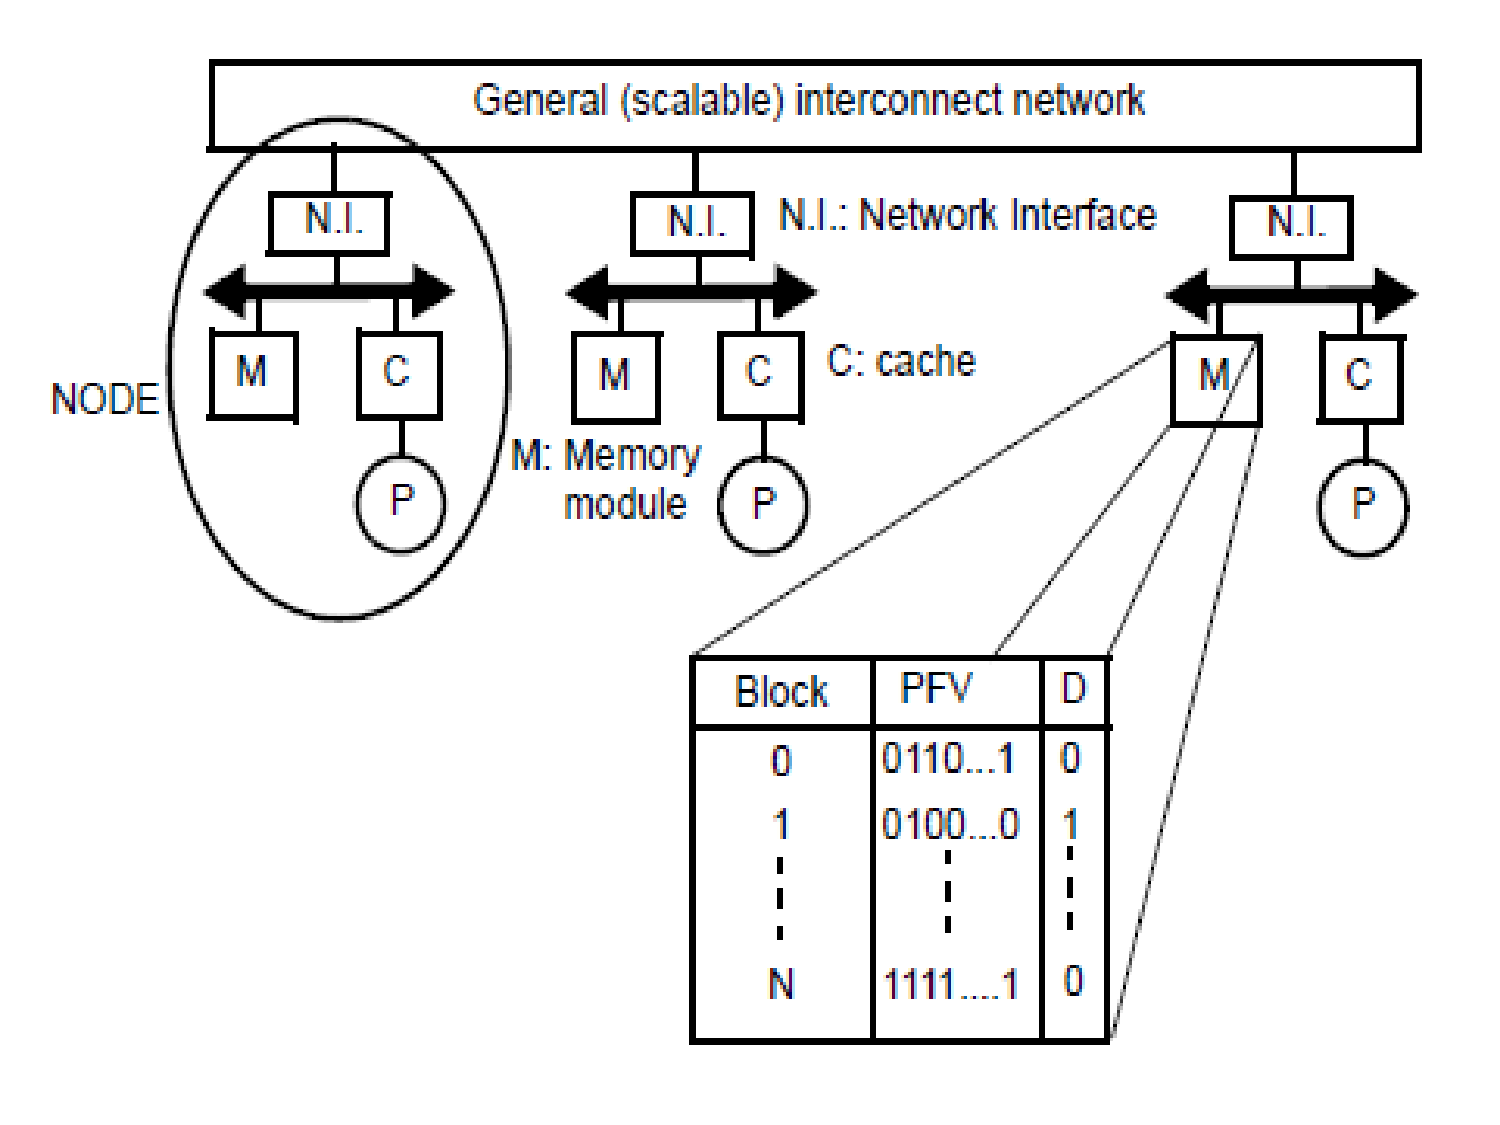
\includegraphics[width=48ex]{FigsInfCoherence/PresenceFlag}
\vspace{-2ex}

A memory block can be in two states: Clean or Dirty. Example:
\begin{itemize}
    \item Block 1 is cached by processor 2 only and is \emp{Dirty},
            i.e., memory is stale and the only valid copy is at a remote node.
    \item Block N is cached by all procs and is \emph{Clean} (mem is up to date).
\end  {itemize}

\end{frame}

\begin{frame}[fragile,t]
\frametitle{cc-NUMA Protocols}

Protocol is similar to MSI-Invalidate (or MSI-Update or MESI),
but without broadcast.
Instead uses only the (protocol) agents:
\begin{itemize}
    \item \emph{Home Node (H)} is the node where the memory block and its 
            directory entry reside,
    \item \emph{Local Node (L)} or requester is the node initiating the request,
    \item \emp{Remote Node (R)} is any other node participating in transaction:
        \begin{itemize}
            \item \emp{Dirty Node (D)} is the node holding the latest modified copy,
            \item \emp{Shared Nodes (S)} are the nodes holding a shared copy. 
        \end  {itemize}
    \item Home may be the same as Local or Dirty.
\end  {itemize}

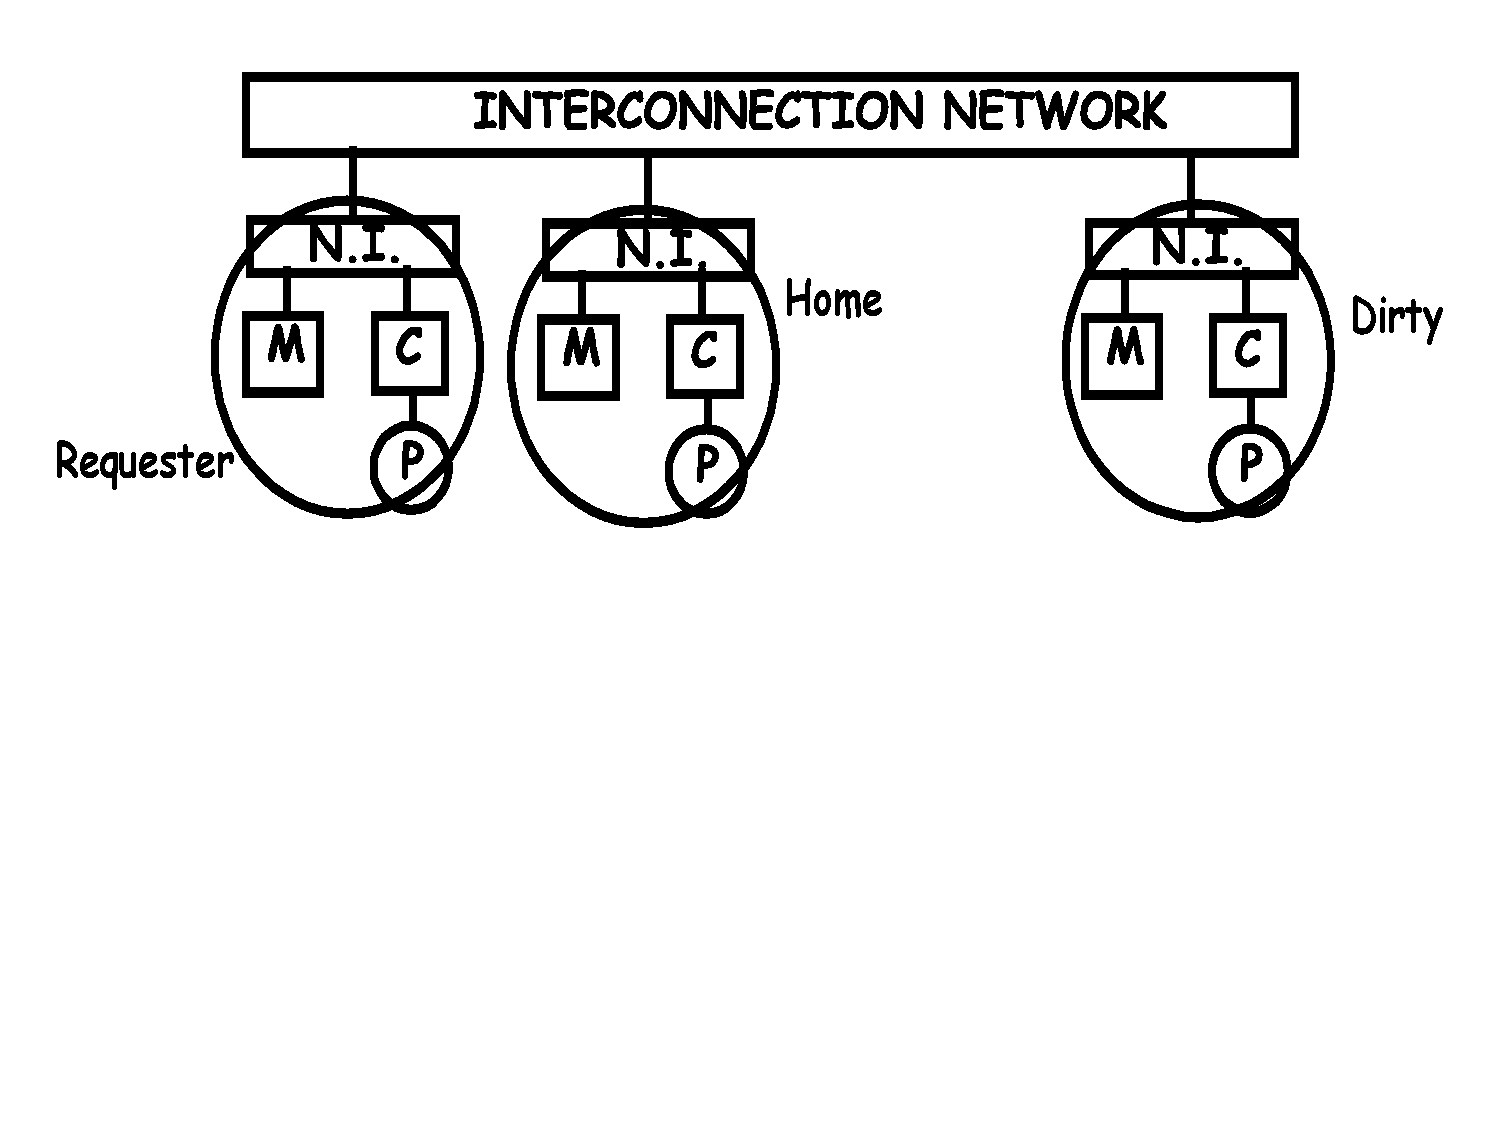
\includegraphics[width=55ex]{FigsInfCoherence/ccNUMA}
\vspace{-1ex}

A block copy can be in two states: Clean or Dirty. Example:
\begin{itemize}
    \item Block 1 is cached by processor 2 only and is Dirty
    \item Block N is cached by all processors and is Clean.
\end  {itemize}

\end{frame}

\begin{frame}[fragile,t]
\frametitle{MSI Invalidate in ccNUMA}

\begin{columns}
\column{0.66\textwidth}
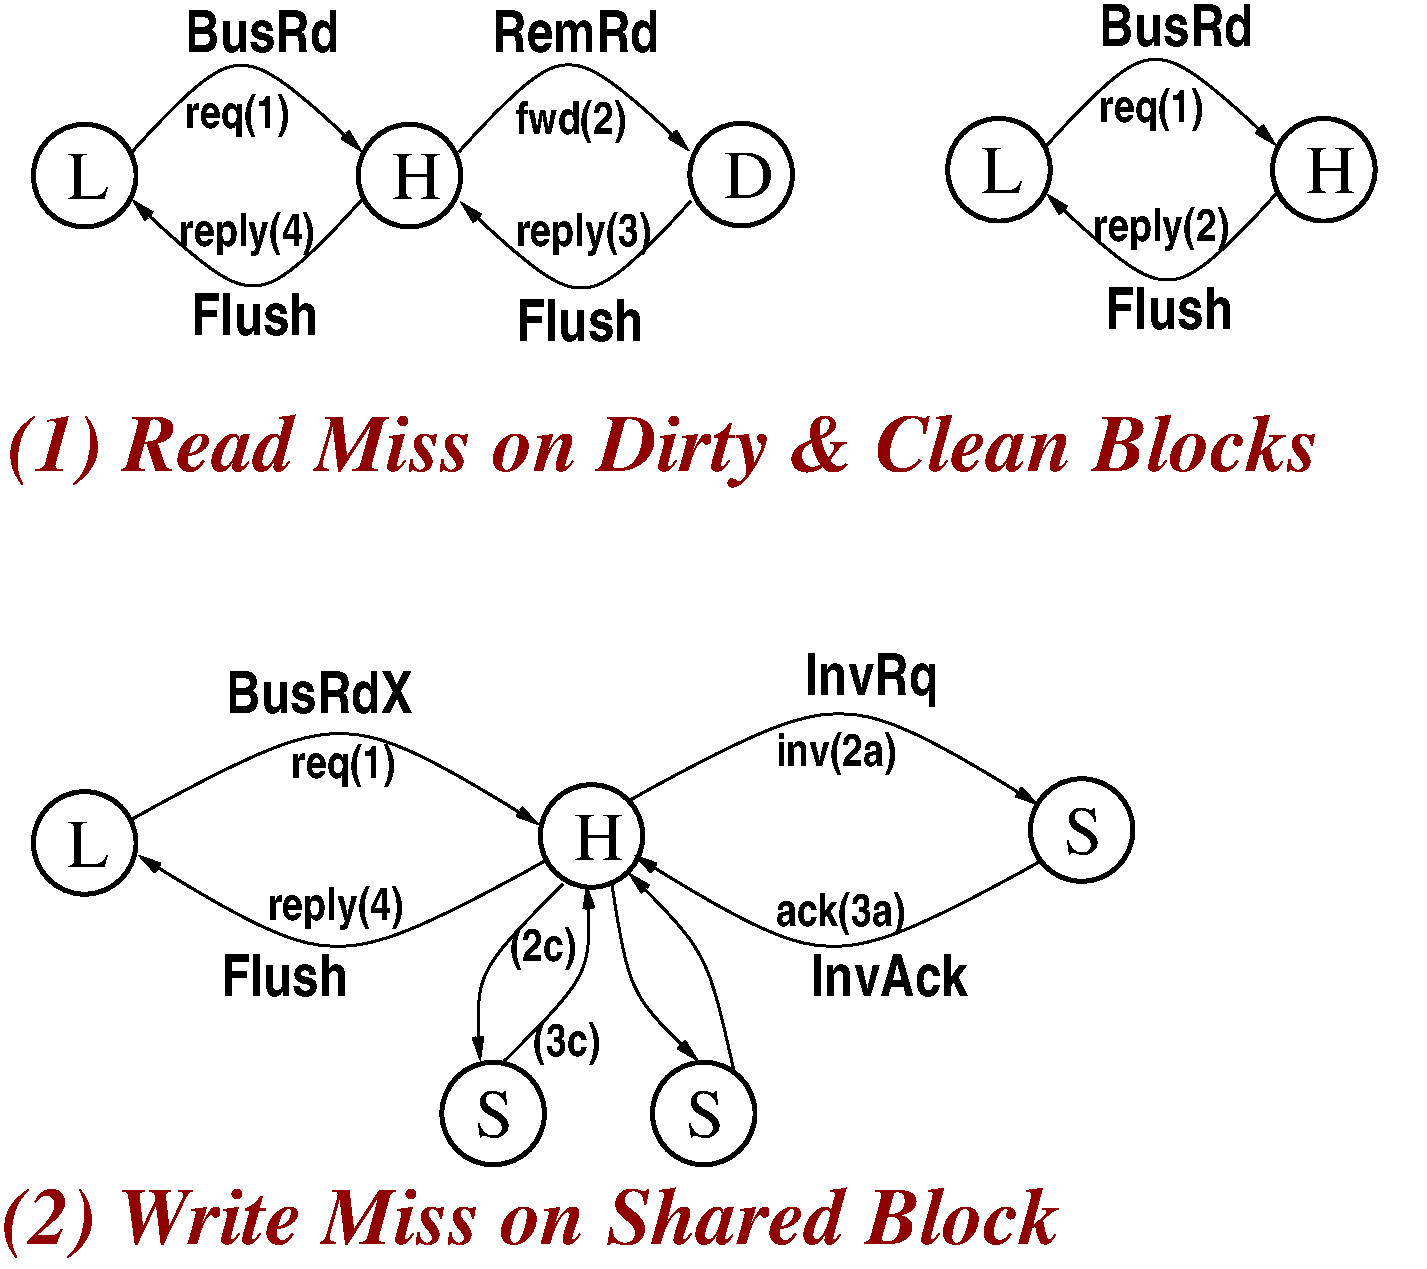
\includegraphics[width=45ex]{FigsInfCoherence/MSIccNUMA}\pause
\column{0.46\textwidth}
\begin{scriptsize}
\begin{itemize}
    \item \emp{Read Miss on Dirty Block:} local node send {\em bus-read} request to host 
                $\Rightarrow$ Since memory (host) is stale,
                   host sends {\em remote-read} request to dirty node, i.e., the only one 
                    set in PFV entry $\Rightarrow$ D sends copy to H $\Rightarrow$ H updates
                    memory and PFV, and sends copy to local (4 hops). 

    \item \emp{Read Miss on Clean Block:} H sends its valid copy to L (2 hops).\smallskip

    \item \emp{Write Miss on Shared Block:} L signals H
            $\Rightarrow$ H sends {\em invalidations} to all sharing nodes
            (found in {\tt PFV}) $\Rightarrow$ When host receives the acks from all 
            S nodes it updates {\tt PFV} (clears all but dirty L) and flushes block to L.
            (4 hops if parallel invs).
    \item \emp{Write Miss on Dirty Block:} dirty node flushes value to L via H.
\end  {itemize}
\end{scriptsize}
\end{columns}
\end{frame}

\begin{frame}[fragile,t]
\frametitle{Block Eviction \& Race Conditions}

\emp{When a block is evicted upon replacement}:
\begin{itemize}
    \item If dirty then OK, i.e., H automatically notified
            by L's write-back.
    \item If no dirty then silent eviction is still correct,
            but affects perform:\\ 
            \emp{Tradeoff} between the overhead of keeping 
            PFV accurate and the overhead of processing 
            useless invalidations.    
\end  {itemize}
\bigskip

Race Conditions: same-block transactions \emp{must not interleave}. \alert{How?}\pause
\begin{itemize}
    \item[1] Home node is the \emph{central arbiter.}
    \item[2] Use a \emph{lock bit per entry} to signal in-progress transaction.
    \item[3] If block-bit set and another transaction then:\\
                \emph{Queueing incomming requests until buffer full then NACK} $\Rightarrow$\\
                reduced latency and bandwidth and simple overflow treatment.
\end  {itemize}
\bigskip

\alert{When should the Lock Bit be cleared/turned off?}
\end{frame}


\begin{frame}[fragile,t]
\frametitle{When to Turn Off the Lock Bit?}

\begin{columns}
\column{0.66\textwidth}
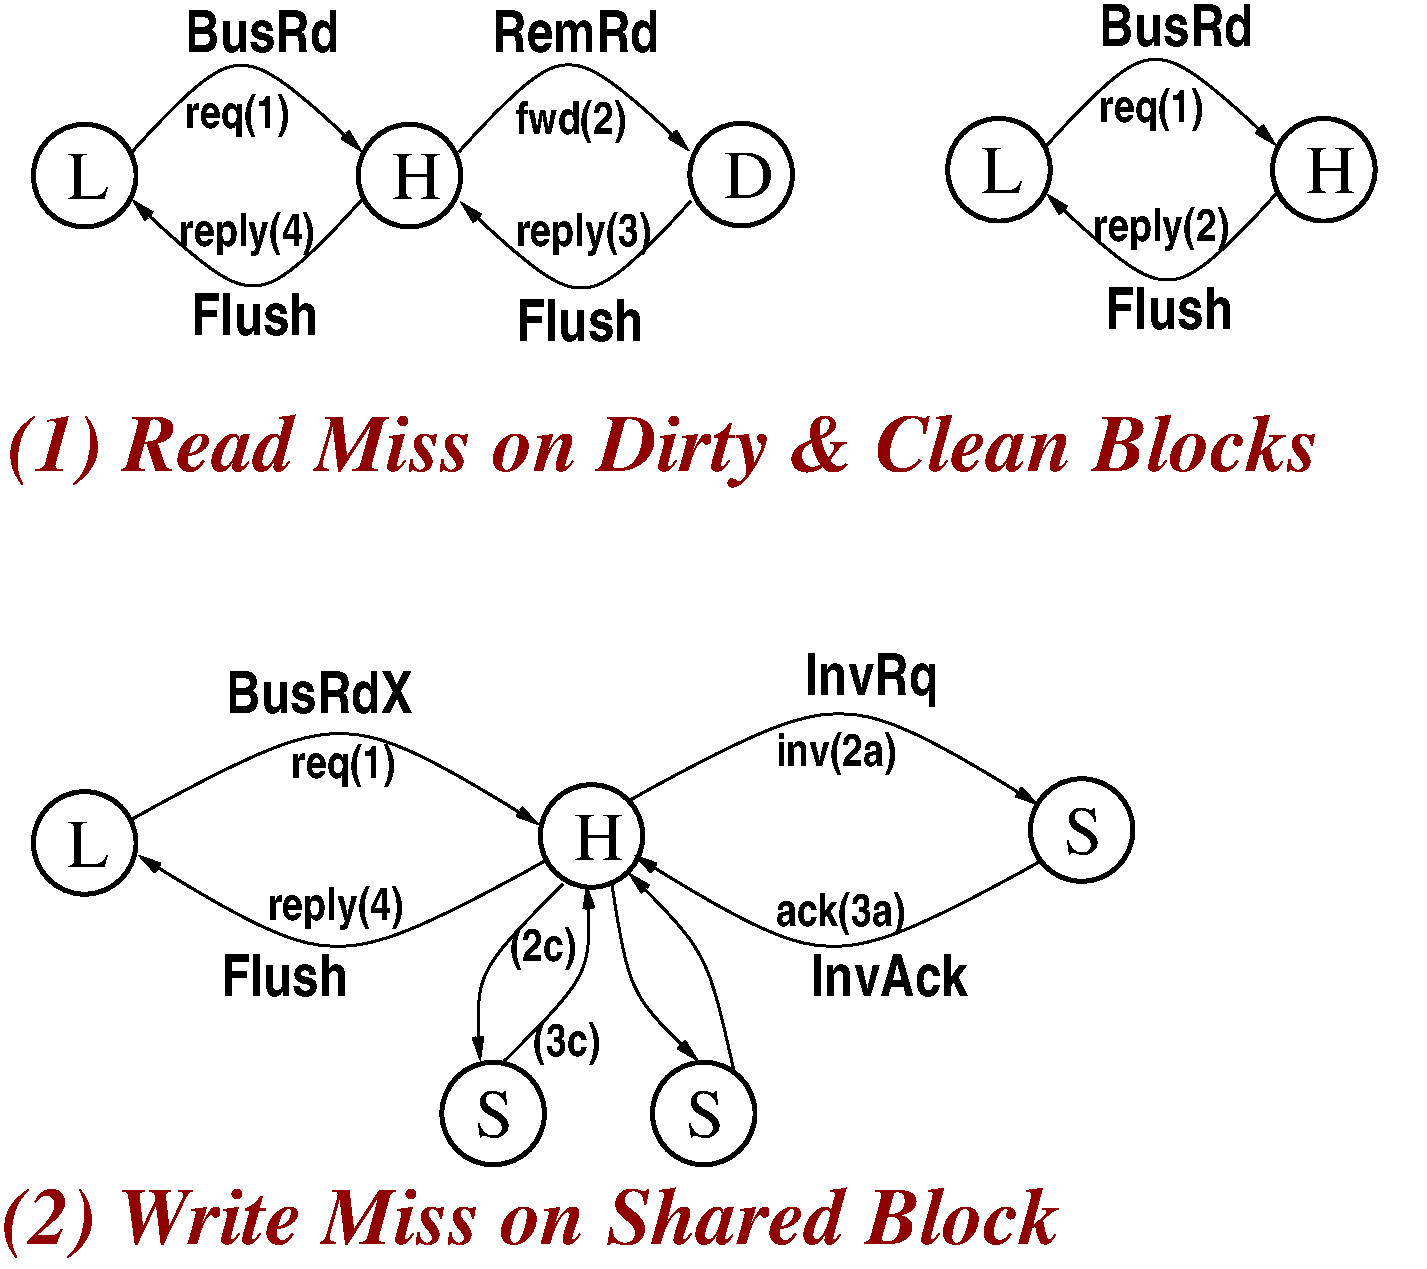
\includegraphics[width=45ex]{FigsInfCoherence/MSIccNUMA}
\column{0.46\textwidth}
Example using Fig \emp{(2)} then \emp{(1)}:
\begin{scriptsize}
\begin{itemize}
    \item The latest time the lock bit can be turned off is
            just before H {\tt Flush}es to L. \alert{Not good enough:}\pause
    \item L is now marked dirty. Assume H receives a read request on 
            the same block and forwards it to L, which is now the 
            dirty node.
    \item If {\tt RemRd} reaches L before the {\tt Flush} from H Then \alert{failure}
            because L does not have the copy yet.  
\end  {itemize}
\end{scriptsize}
\bigskip
\emph{A Solution:} L acknowledges to H the end of transaction,
        i.e., that it has received the {\tt Flush}. After
        acknowledgement H can safely turn off the Lock Bit! 
\end{columns}

\end{frame}


\begin{frame}[fragile,t]
\frametitle{Standard DASH System: Optimizing Latencies}

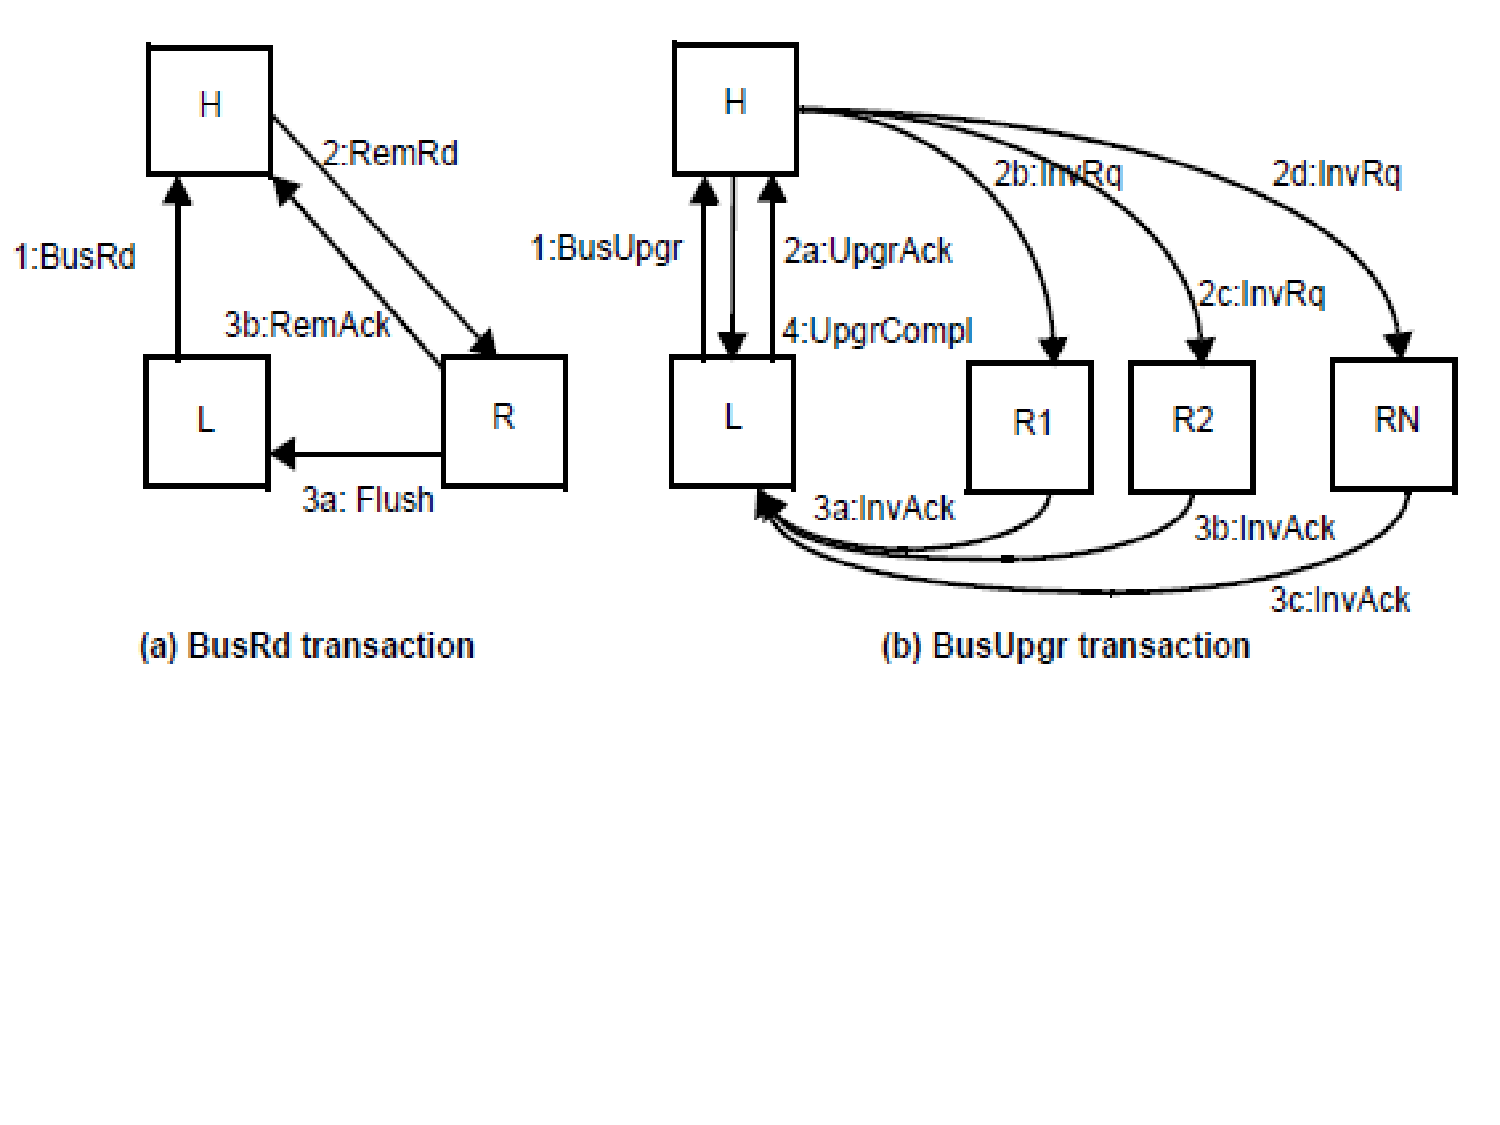
\includegraphics[width=55ex]{FigsInfCoherence/RedLatencyCCNUMA}
\vspace{-15ex}

Baseline Protocol needs at worst 4 hops. 
\emph{Can make it in THREE}:\pause
\begin{itemize}
    \item[1] Request is sent to Home
    \item[2] H redirects request to remote nodes.\\ 
             In (b) H also sends L the \# of remotes via {\tt 2a:UpgrAck}
    \item[3] Remote responds to L (L now knows when all have responded).\medskip
    \item[4] L notifies transaction completed, \emp{off the critical access path}
\end  {itemize}

\end{frame}

\begin{frame}[fragile,t]
\frametitle{Memory Requirements of Directory Protocols}

Assume $N$ nodes (processors), and $M$ memory blocks per node.
\bigskip


\emp{Total Presence-Flag Vector (PFV) Directory Size:} $M\times N\times$\alert{$N$}\\
\alert{grows linearly with N, hence a serious scalability concern.}\\
($N$ node directories, each with $M$ entries, and each entry has $N$ bits.)
\bigskip

One Alternative is Limited Pointer Protocol (LPP):
\begin{itemize}
    \item Each entry maintains $i$ pointers, each represented on {\tt log $N$} bits\\
            (instead of $N$ bits in PFV).
    \item \emp{Total LPP Directory Size:} $M\times N\times i \times$\emph{$log N$}\\ 
            \emph{grows logarithmically (sublinearly) with N} (because $i$ is constant) 
    \item Failback: resort to broadcast when the directory pointers are exhausted.
\end  {itemize}

\end{frame}


\begin{frame}[fragile,t]
\frametitle{Other Scalable Protocols}

\emp{Coarse Vector Schemes:} presence flags identify groups rather than individual nodes.
\smallskip

\emp{Directory Cache}, i.e., at cache rather than main memory level $\Rightarrow$
memory overhead is proportional to cache size (leverages locality).\medskip 

\emp{Cache-Centric Directories, for example Scalable Coherent Interface:}

\begin{columns}
\column{0.58\textwidth}
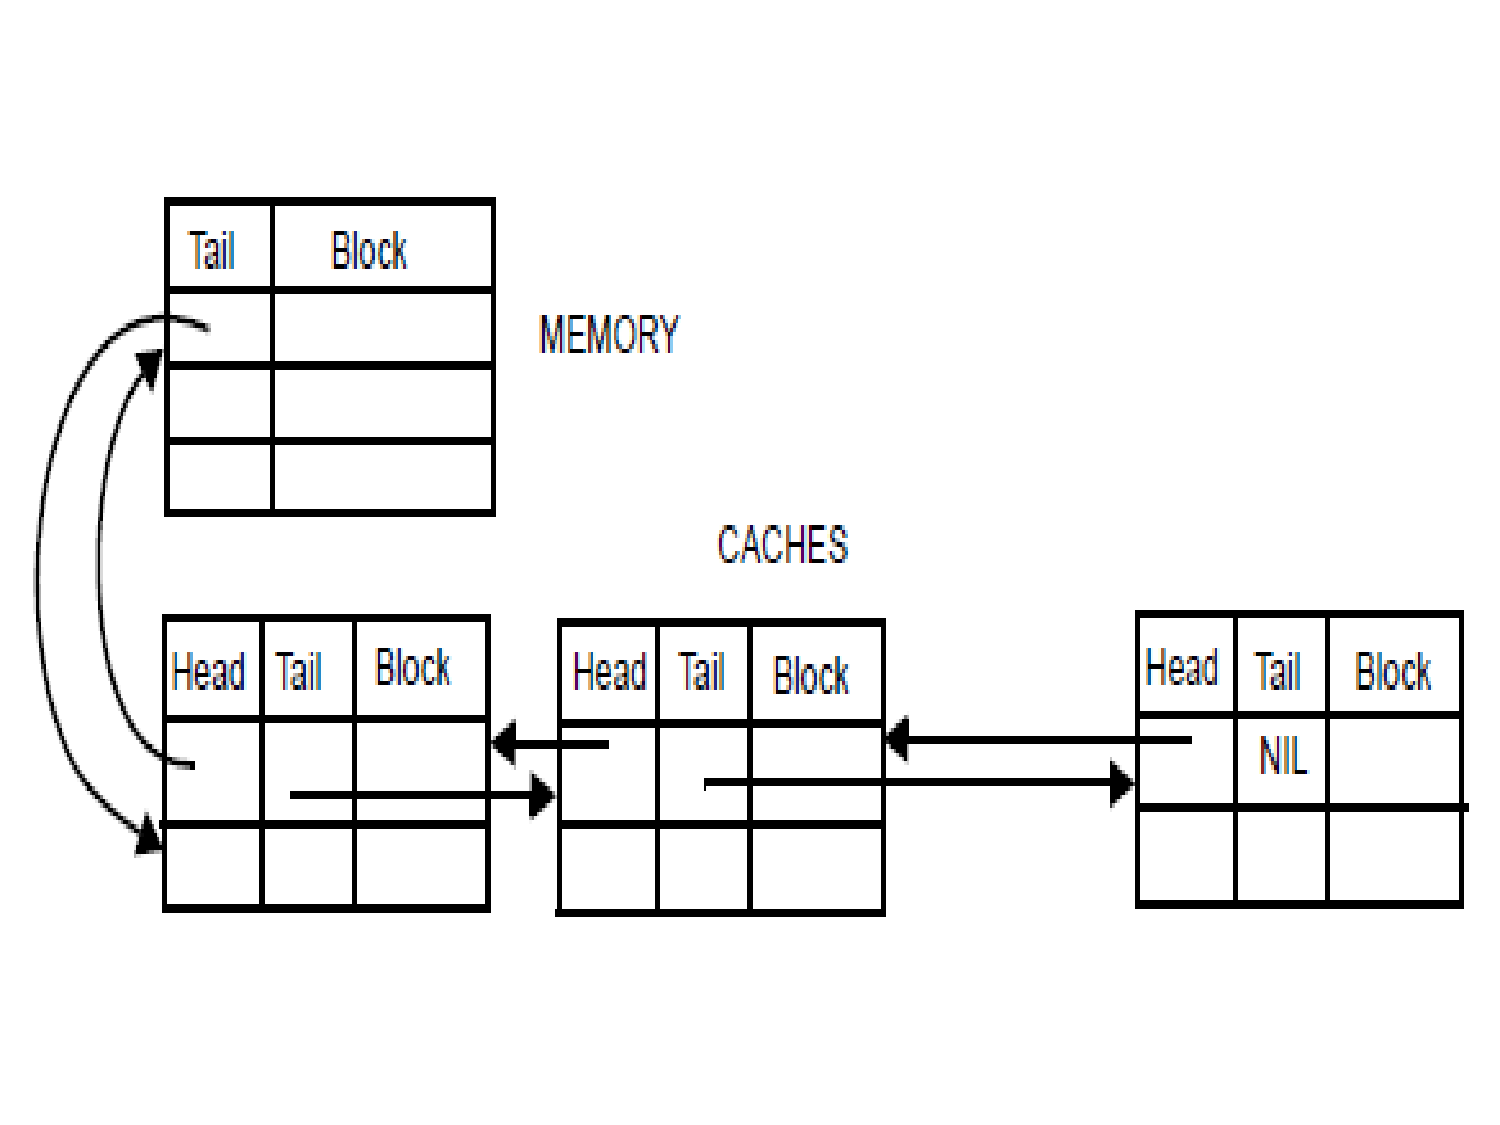
\includegraphics[width=40ex]{FigsInfCoherence/CacheCentricProt}
\column{0.48\textwidth}
\begin{scriptsize}
\begin{itemize}
    \item Directory Entry: Copies of the same memory block in different (private) 
            caches are linked via a double-linked list (implemented in cache-hardware)
    \item  \emph{Directory size proportional with the total (private) cache size},
            rather than to the main memory size as in PFV.
    \item \emp{Latency of {\tt BusRdX/BusUpgr} larger} than PFV because invalidations do not
            go in parallel (list requires sequential traversal).
    \item Bandwidth is comparable to PFV.
\end  {itemize}
\end{scriptsize}
\end{columns}

\end{frame}


\begin{frame}[fragile,t]
\frametitle{Hierarchical Systems}

\vspace{-7ex}
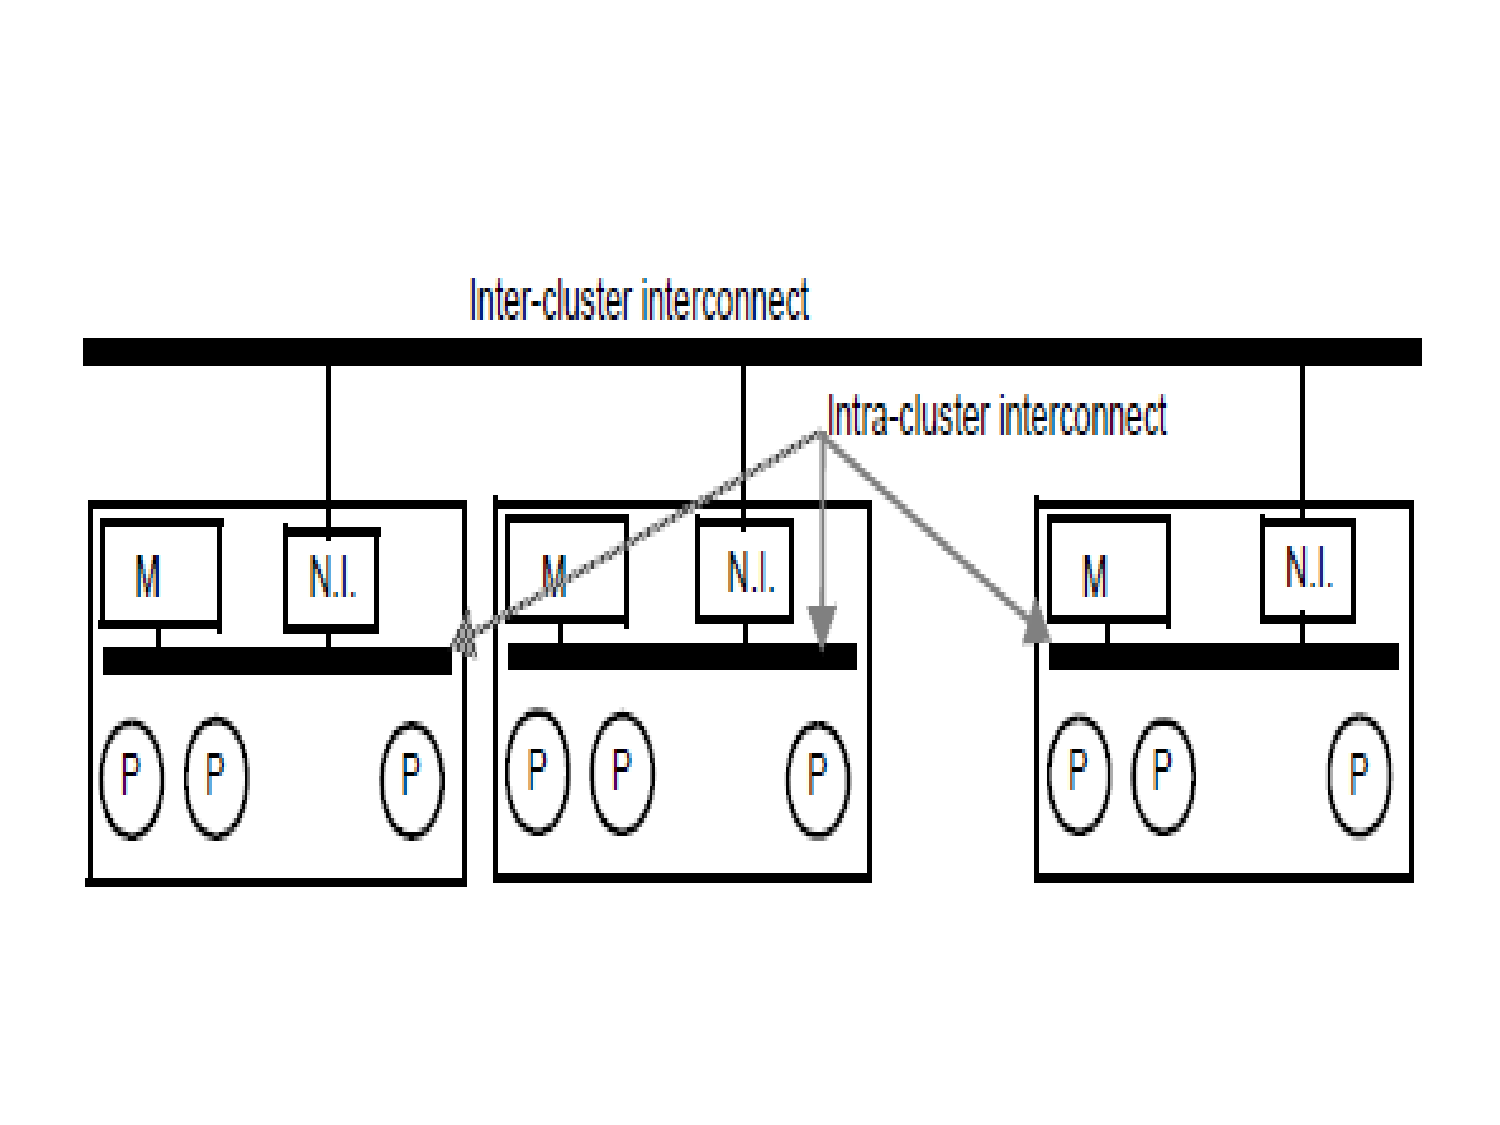
\includegraphics[width=44ex]{FigsInfCoherence/HierarchSys}
\vspace{-5ex}

Instead of scaling in a flat configuration, one can form clusters
in a hierarchical organization.   Relevant inside, as well as 
across chip multiprocs!
\bigskip

\emp{Coherence Options:}
\begin{itemize}
    \item Intra-Cluster Coherence: snoopy / directory
    \item Inter-Cluster Coherence: snoopy / directory
    \item \alert{Tradeoffs} between memory overhead and performance to maintain coherence.
\end  {itemize}
\end{frame}


\end{document}
